\documentclass{article}
\author{Gabriel Haruo Hanai Takeuchi - NUSP: 13671636}
\title{MAC0210 - Relatório do EP2}
\date{}

\usepackage[utf8]{inputenc}
\usepackage[a4paper, margin=2cm]{geometry}
\usepackage[skip=5pt]{parskip}
\usepackage{amsmath, amssymb, amsthm}
\usepackage{graphicx}
\usepackage{float}
\usepackage{subcaption}
\usepackage{hyperref}

\begin{document}
\maketitle

\section{Implementação}

A seguir serão explicitados alguns pontos na implementação das 
\textit{function files} requisitadas.

\subsection{compress}

A função \texttt{compress.m} é a mais simples entre as três. Pega-se o
tamanho da imagem de entrada e cria-se uma máscara que filtra todas as
colunas e linhas, de 1 a $p$, múltiplas de $k+1$. Essa máscara é aplicada
na matriz da imagem original, resultando em uma comprimida.

\subsection{decompress}

Na função \texttt{decompress.m}, foram seguidas as instruções do enunciado
para os métodos bilinear e bicúbico (todas as matrizes coeficientes,
derivadas parciais, etc). Os casos das bordas foi lidado facilmente com alguns
\texttt{if statements}. Além disso, foram criadas funções auxiliares que
calculam derivadas parciais.

Em ambos os métodos, itera-se pelas linhas e colunas. Para cada pixel,
é calculada uma matriz de coeficientes (a matriz mais computacionalmente
custosa é para o método bicúbico), além de uma iteração ao redor do pixel
mencionado anteriormente.

\subsection{calculateError}

Na função \texttt{calculateError.m}, foi seguido exatamente o requisitado.
Itera-se pelas linhas, colunas, e para cada pixel, há o cálculo do erro de
cada canal RGB. 

\subsection{Conclusão}

Em termos gerais, os algoritmos de processamento de imagem em Octave são
custosos e demorados em tempo de execução. Isto pois o cálculo de matrizes
é computacionalmente exigente. Não obstante, os resultados são espetaculares
para os olhos. 

\section{Experimentos}

A seguir, serão apresentados os experimentos com diversas funções,
algumas de classe $C^2$ e outras não necessariamente.

\subsection{Funções senoidais} \label{subsec:funcoesSenoidais}

Esta é a função requisitada pelo enunciado na \textit{Parte 1 - O zoológico}.

A função
\begin{equation} \label{eq:funcaoSenoidalAntes}
  f(x,y) = \Biggl( \sin(x)
  , \dfrac{\sin(y) + \sin(x)}{2}
  , \sin(x) \Biggr)
\end{equation}
foi convertida para
\begin{equation}
  f(x,y) = \Biggl( (\sin(x) + 1) \dfrac{255}{2}
  , \Bigl( \frac{\sin(y) + \sin(x)}{2} + 1 \Bigr) \dfrac{255}{2}
  , (\sin(x) + 1) \dfrac{255}{2} \Biggr)
  \label{eq:funcaoSenoidalDepois}
\end{equation}
Isto pois a imagem de cada função da equação \ref{eq:funcaoSenoidalAntes}
é $[-1,1]$. Como os valores de cada canal RGB variam entre [0,255],
então o fator de conversão é somar $1$ e multiplicar por
$255/2$.

\subsubsection[Usando h=1]{Usando $h=1$} \label{subsubsec:senoidal-h=1}
Usando $k=3$ e $h=1$, as imagens resultantes foram

\begin{figure}[ht]
  \centering
  \begin{subfigure}{0.23\textwidth}
    \centering
    
\includegraphics[width=\textwidth]{senoidal/senoidal.png}
    \caption{Original}
  \end{subfigure}%
  \hfill
  \begin{subfigure}{0.23\textwidth}
    \centering
    
\includegraphics[width=\textwidth]{senoidal/h-1/compressed.png}
    \caption{Comprimida}
  \end{subfigure}%
  \hfill
  \begin{subfigure}{0.23\textwidth}
    \centering
    
\includegraphics[width=\textwidth]{senoidal/h-1/decompressed-bilinear.png}
    \caption{Bilinear}
  \end{subfigure}%
  \hfill
  \begin{subfigure}{0.23\textwidth}
    \centering
    
\includegraphics[width=\textwidth]{senoidal/h-1/decompressed-bicubica.png}
    \caption{Bicúbica}
  \end{subfigure}
  \caption{Imagem original (1024 pixels), comprimida (256 pixels) e descomprimidas (1024 pixels)}
\end{figure}

e os erros foram 0.016470 para bilinear e 0.016539 para bicúbica. Erros
semelhantes.

\subsubsection[Usando h=10]{Usando $h=10$}

Usando $k=3$ e $h=10$, as imagens resultantes foram

\begin{figure}[ht]
  \centering
  \begin{subfigure}{0.23\textwidth}
    \centering
    
\includegraphics[width=\textwidth]{senoidal/senoidal.png}
    \caption{Original}
  \end{subfigure}%
  \hfill
  \begin{subfigure}{0.23\textwidth}
    \centering
    
\includegraphics[width=\textwidth]{senoidal/h-10/compressed.png}
    \caption{Comprimida}
  \end{subfigure}%
  \hfill
  \begin{subfigure}{0.23\textwidth}
    \centering
    
\includegraphics[width=\textwidth]{senoidal/h-10/decompressed-bilinear.png}
    \caption{Bilinear}
  \end{subfigure}%
  \hfill
  \begin{subfigure}{0.23\textwidth}
    \centering
    
\includegraphics[width=\textwidth]{senoidal/h-10/decompressed-bicubica.png}
    \caption{Bicúbica}
  \end{subfigure}
  \caption{Imagem original (1024 pixels), comprimida (256 pixels) e descomprimidas (1024 pixels)}
\end{figure}

e os erros foram 0.016470 para bilinear e 0.025466 para bicúbica.
\subsubsection{Observações}

Note que a equação \ref{eq:funcaoSenoidalDepois} é de classe $C^2$,
e portanto, a compressão e descompressão se comportam com erros relativamente
baixos, com 2 casas decimais.
Entretanto,  houve um salto entre a diferença dos erros bilinear e bicúbico
para $h=10$ e $h=1$. O delta na seção \ref{subsubsec:senoidal-h=1} é igual a 
$|0.016470 - 0.016539| = 0.000069$, enquanto nessa é $|0.016470 - 0.025466|
= 0.008996$.


\subsection{Funções polinomiais simples}

A função
\begin{equation}
  f(x,y) = \Biggl( 255 \Bigl(\dfrac{150-x}{y-x}\Bigr) , 255 \Bigl(\dfrac{150-x}{y-x}\Bigr)^2 , 255 \Bigl(\dfrac{150-x}{y-x}\Bigr)^3 \; \Biggr) \label{eq:funcaoPolinomial}
\end{equation}

\subsubsection[Usando h=1]{Usando $h=1$}

Usando $k=3$ e $h=1$, as imagens resultantes foram

\begin{figure}[ht]
  \centering
  \begin{subfigure}{0.23\textwidth}
    \centering
    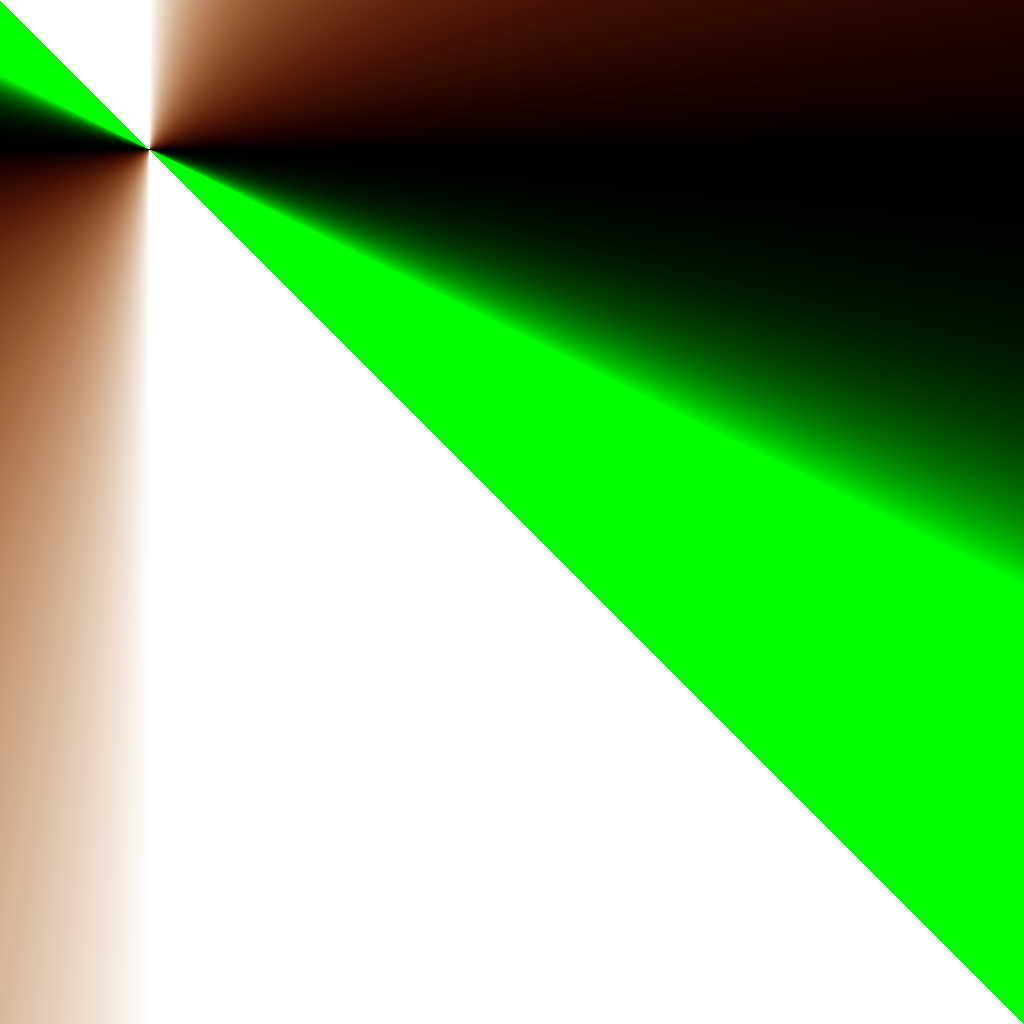
\includegraphics[width=\textwidth]{polinomial/polinomial.png}
    \caption{Original}
  \end{subfigure}%
  \hfill
  \begin{subfigure}{0.23\textwidth}
    \centering
    
\includegraphics[width=\textwidth]{polinomial/h-1/compressed.png}
    \caption{Comprimida}
  \end{subfigure}%
  \hfill
  \begin{subfigure}{0.23\textwidth}
    \centering
    
\includegraphics[width=\textwidth]{polinomial/h-1/decompressed-bilinear.png}
    \caption{Bilinear}
  \end{subfigure}%
  \hfill
  \begin{subfigure}{0.23\textwidth}
    \centering
    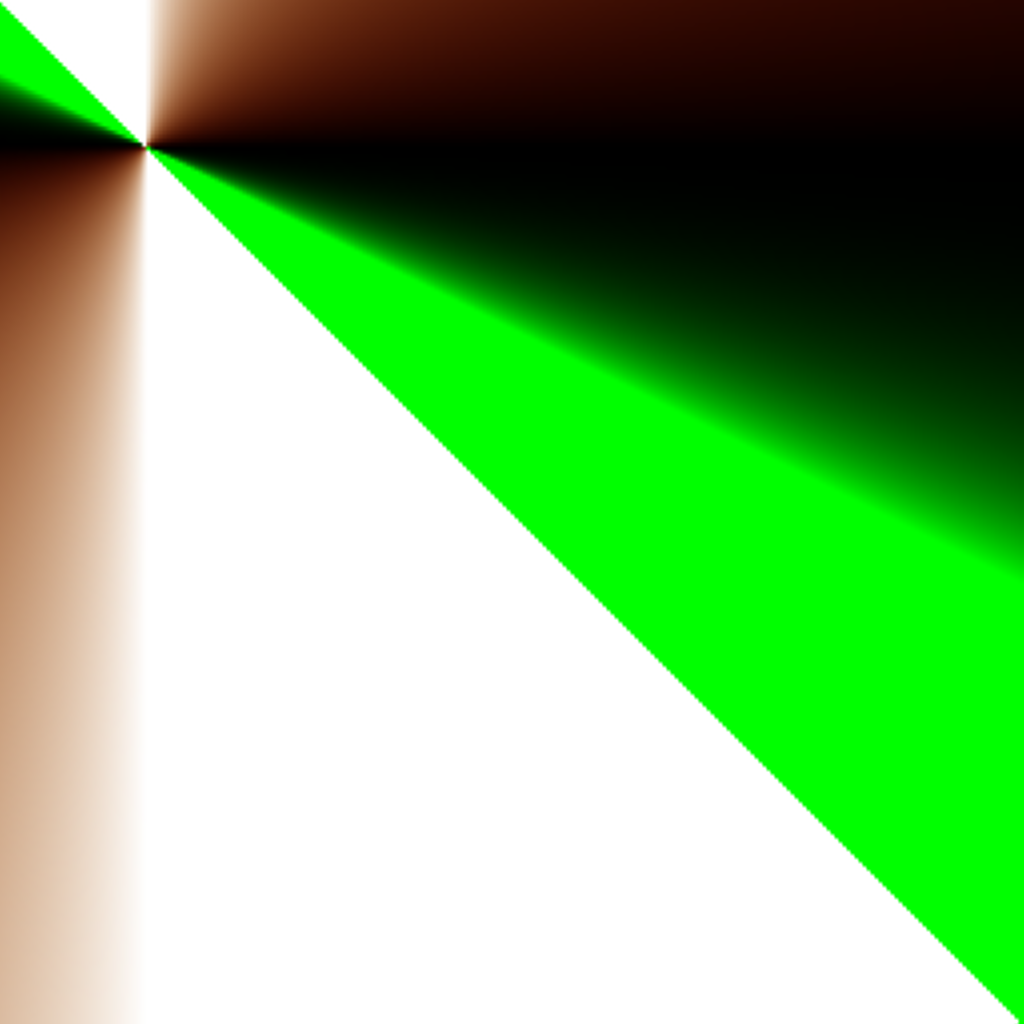
\includegraphics[width=\textwidth]{polinomial/h-1/decompressed-bicubica.png}
    \caption{Bicúbica}
  \end{subfigure}
  \caption{Imagem original (1024 pixels), comprimida (256 pixels) e descomprimidas (1024 pixels)}
\end{figure}

\newpage

e os erros foram 0.025576 para bilinear e 0.025724 para bicúbica.

\subsubsection[Usando h=10]{Usando $h=10$}

Usando $k=3$ e $h=10$, as imagens resultantes foram

\begin{figure}[ht]
  \centering
  \begin{subfigure}{0.23\textwidth}
    \centering
    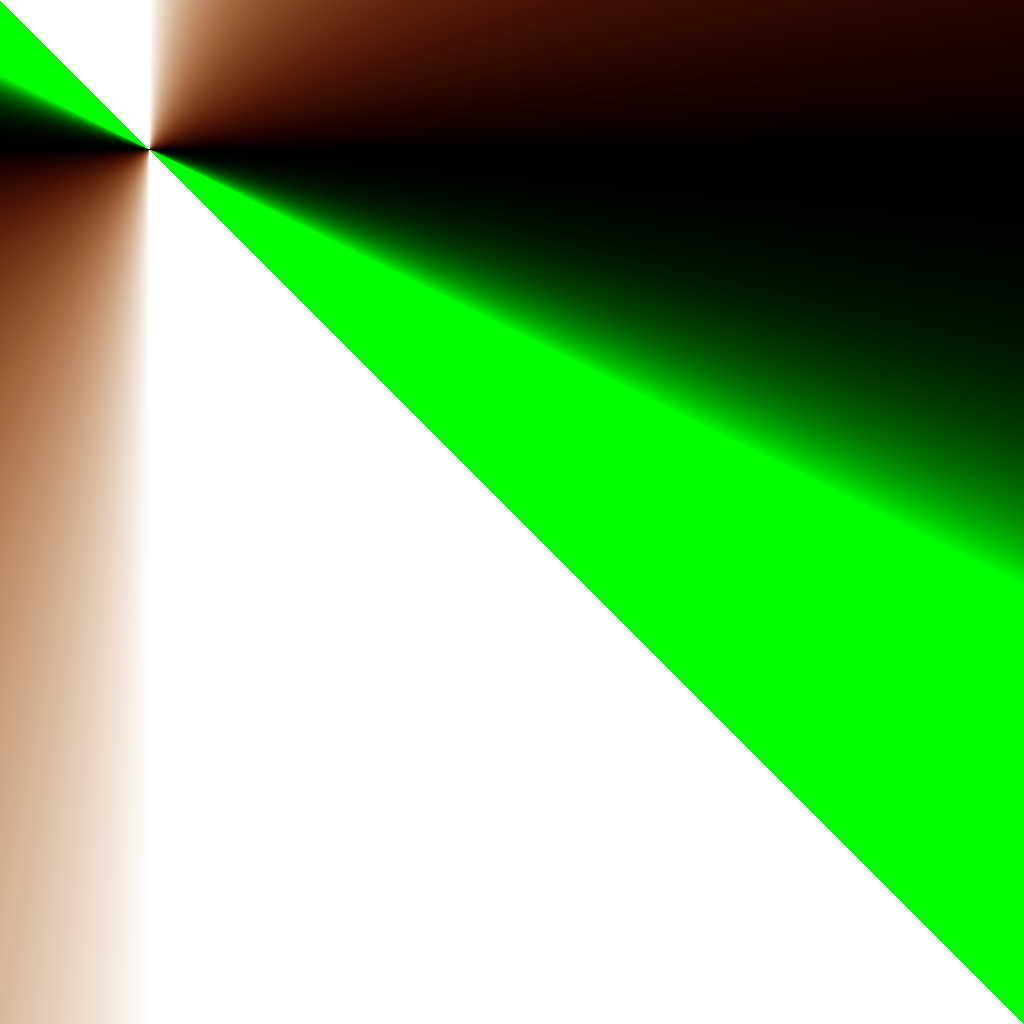
\includegraphics[width=\textwidth]{polinomial/polinomial.png}
    \caption{Original}
  \end{subfigure}%
  \hfill
  \begin{subfigure}{0.23\textwidth}
    \centering
    
\includegraphics[width=\textwidth]{polinomial/h-10/compressed.png}
    \caption{Comprimida}
  \end{subfigure}%
  \hfill
  \begin{subfigure}{0.23\textwidth}
    \centering
    
\includegraphics[width=\textwidth]{polinomial/h-10/decompressed-bilinear.png}
    \caption{Bilinear}
  \end{subfigure}%
  \hfill
  \begin{subfigure}{0.23\textwidth}
    \centering
    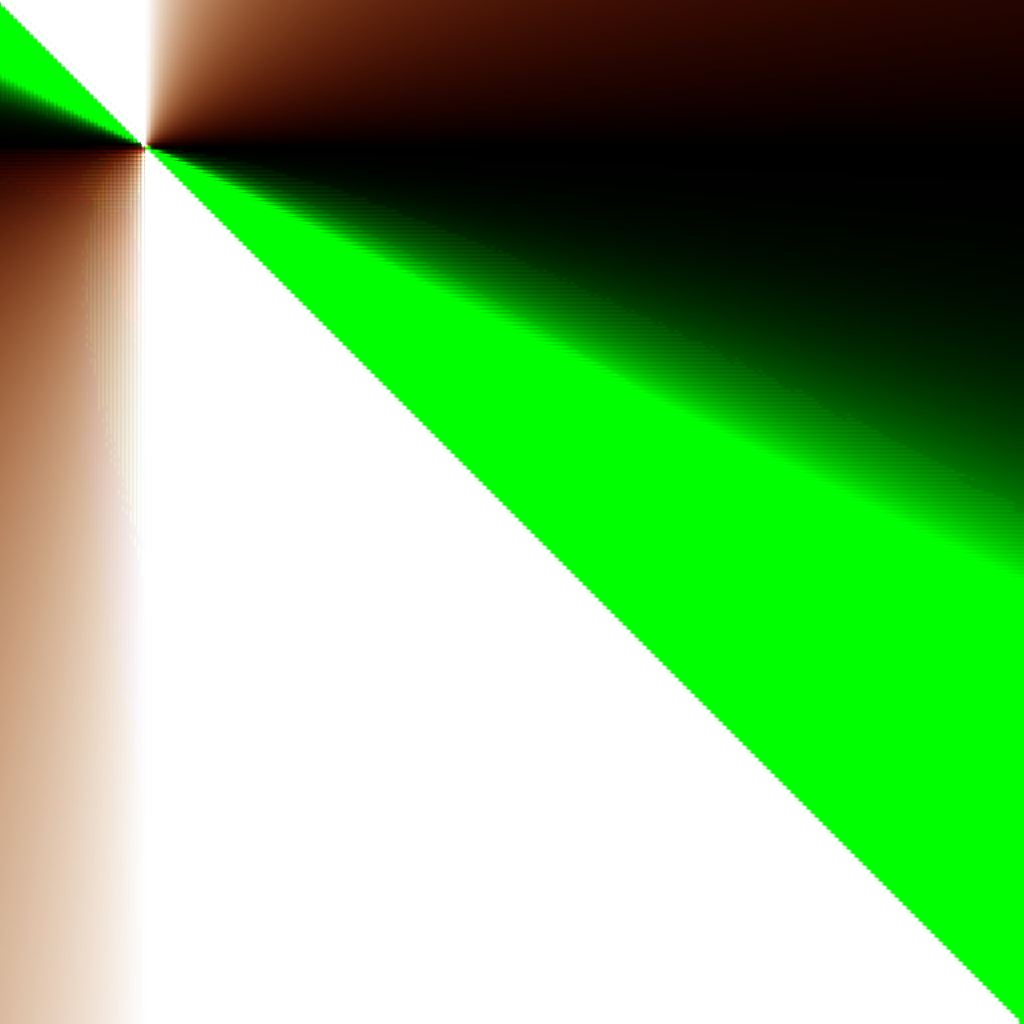
\includegraphics[width=\textwidth]{polinomial/h-10/decompressed-bicubica.png}
    \caption{Bicúbica}
  \end{subfigure}
  \caption{Imagem original (1024 pixels), comprimida (256 pixels) e descomprimidas (1024 pixels)}
\end{figure}

e os erros foram 0.025577 para bilinear e 0.027910 para bicúbica.

\subsubsection{Observações}

Note que, semelhante à seção \ref{subsec:funcoesSenoidais},
a equação \ref{eq:funcaoPolinomial} é de classe $C^2$. O erro,
mesmo sendo maior que o da seção \ref{subsec:funcoesSenoidais},
ainda é possível perceber nitidez entre as imagens.

\subsection{Funções preto e branco}

A função 
\begin{equation}
  f(x,y) = \begin{cases}
    (255, 255, 255) &\text{se } x \equiv 0 \pmod 7 \text{ ou } y \equiv 0 \pmod{23} \\
    (0, 0, 0) &\text{caso contrário}  
  \end{cases}
\end{equation}
gera uma imagem com fundo preto e retângulos brancos.
Note que essa função não é de classe $C^2$, muito menos contínua.

\subsubsection[Usando h=7]{Usando $h=7$}

Usando $k=3$ e $h=7$, as imagens resultantes foram

\begin{figure}[ht]
  \centering
  \begin{subfigure}{0.23\textwidth}
    \centering
    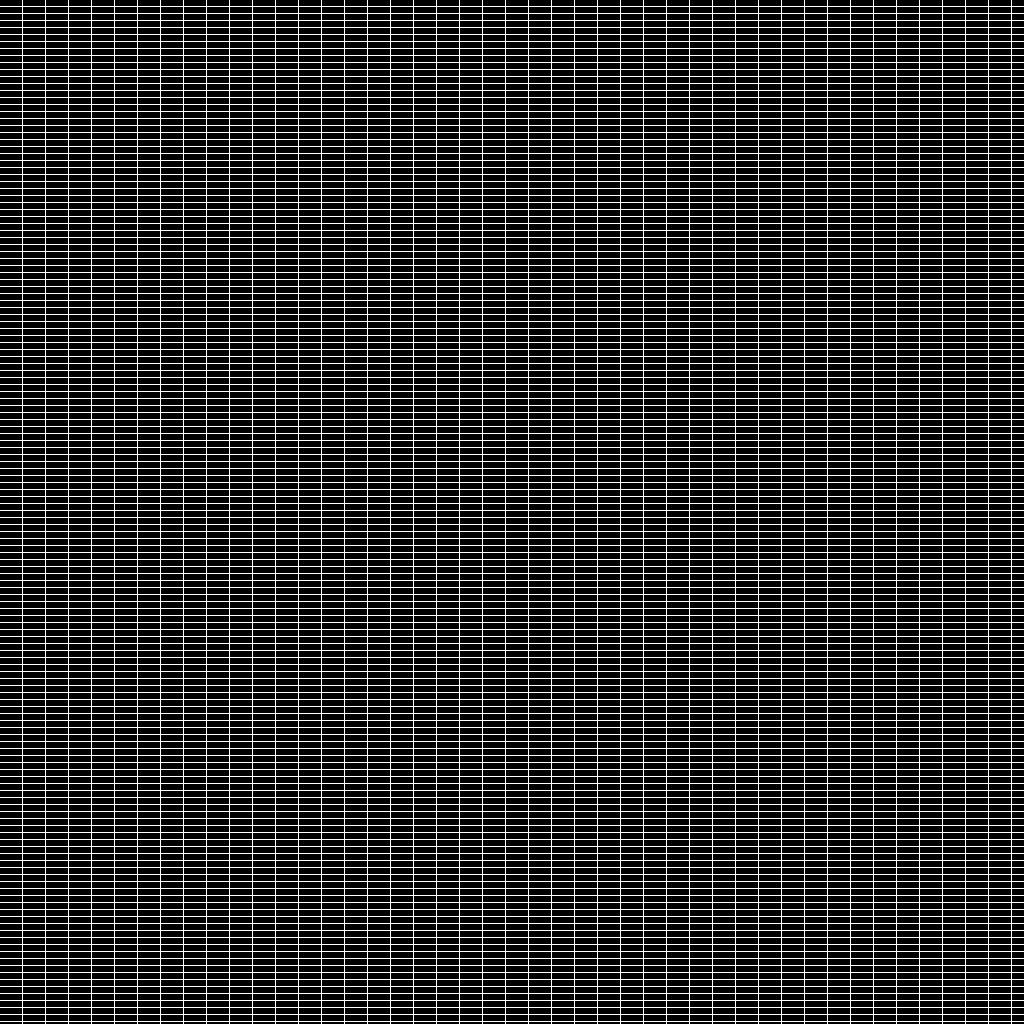
\includegraphics[width=\textwidth]{pb/pb.png}
    \caption{Original}
  \end{subfigure}%
  \hfill
  \begin{subfigure}{0.23\textwidth}
    \centering
    
\includegraphics[width=\textwidth]{pb/compressed.png}
    \caption{Comprimida}
  \end{subfigure}%
  \hfill
  \begin{subfigure}{0.23\textwidth}
    \centering
    
\includegraphics[width=\textwidth]{pb/decompressed-bilinear.png}
    \caption{Bilinear}
  \end{subfigure}%
  \hfill
  \begin{subfigure}{0.23\textwidth}
    \centering
    
\includegraphics[width=\textwidth]{pb/decompressed-bicubica.png}
    \caption{Bicúbica}
  \end{subfigure}
  \caption{Imagem original (1024 pixels), comprimida (256 pixels) e descomprimidas (1024 pixels)}
\end{figure}
\newpage
e os erros foram 0.423 para bilinear e 0.423 para bicúbica.

\subsubsection{Observações}

Note que foram geradas imagens totalmente pretas na compressão e descompressão.
Sendo breve, o processo não funciona bem para imagens binárias, pretas e brancas,
desse tipo.

\subsection{Funções que geram um gradiente}

A função
\begin{equation}
  f(x,y) = \Biggl( 255 \dfrac{x}{1024} , 255 \dfrac{y}{1024}, 1 \Biggr)
\end{equation}
gera um gradiente linear.

\subsubsection[Usando h=1]{Usando $h=1$}

Usando $k=3$ e $h=1$, as imagens resultantes foram

\begin{figure}[ht]
  \centering
  \begin{subfigure}{0.23\textwidth}
    \centering
    
\includegraphics[width=\textwidth]{gradiente/gradiente.png}
    \caption{Original}
  \end{subfigure}%
  \hfill
  \begin{subfigure}{0.23\textwidth}
    \centering
    
\includegraphics[width=\textwidth]{gradiente/compressed.png}
    \caption{Comprimida}
  \end{subfigure}%
  \hfill
  \begin{subfigure}{0.23\textwidth}
    \centering
    
\includegraphics[width=\textwidth]{gradiente/decompressed-bilinear.png}
    \caption{Bilinear}
  \end{subfigure}%
  \hfill
  \begin{subfigure}{0.23\textwidth}
    \centering
    
\includegraphics[width=\textwidth]{gradiente/decompressed-bicubica.png}
    \caption{Bicúbica}
  \end{subfigure}
  \caption{Imagem original (1024 pixels), comprimida (256 pixels) e descomprimidas (1024 pixels)}
\end{figure}
e os erros foram 2.6067e-03 para bilinear e 2.6067e-03 para bicúbica.

\subsubsection{Observações}

São erros bem mais baixos comparado às outras funções, e perceptível na
nitidez das imagens.

\subsection[Funções diferenciáveis mas não de classe C1]{Funções diferenciáveis mas não de classe $C^1$}

Esta subseção foi baseada \href{https://en.wikipedia.org/wiki/Smoothness}{neste}
artigo da Wikipedia sobre \textit{Smoothness of a function}.

A função
\begin{equation}
  f(x,y) = \begin{cases}
  (0, 0, 0) & \mbox{ se } x = 0 \mbox{ e } y = 0 \\
  \Biggl(
    \dfrac{255}{p} x^2 sin\Bigl(\frac{1}{x}\Bigr)
  , \dfrac{255}{p} y^2 \sin \Bigl( \frac{1}{x} \Bigr)
  , \dfrac{255}{p} (x+y)
  \Biggr) &\text{ caso contrário}
  \end{cases}
\end{equation}
gera uma imagem com uma divisão arredondada, característica de funções senoidais.

Obs.: $p$ é a largura (ou altura) da imagem original.

\subsubsection[Usando h=1]{Usando $h=1$}

Usando $k=3$ e $h=1$, as imagens resultantes foram

\begin{figure}[ht]
  \centering
  \begin{subfigure}{0.23\textwidth}
    \centering
    
\includegraphics[width=\textwidth]{notc1/notc1.png}
    \caption{Original}
  \end{subfigure}%
  \hfill
  \begin{subfigure}{0.23\textwidth}
    \centering
    
\includegraphics[width=\textwidth]{notc1/compressed.png}
    \caption{Comprimida}
  \end{subfigure}%
  \hfill
  \begin{subfigure}{0.23\textwidth}
    \centering
    
\includegraphics[width=\textwidth]{notc1/decompressed-bilinear.png}
    \caption{Bilinear}
  \end{subfigure}%
  \hfill
  \begin{subfigure}{0.23\textwidth}
    \centering
    
\includegraphics[width=\textwidth]{notc1/decompressed-bicubica.png}
    \caption{Bicúbica}
  \end{subfigure}
  \caption{Imagem original (1024 pixels), comprimida (256 pixels) e descomprimidas (1024 pixels)}
\end{figure}
e os erros foram 4.7175e-03 para bilinear e 4.5450e-03 para bicúbica.

\subsubsection{Observações}

A imagem original é linda, e os erros também são lindamente baixos. Mesmo uma
das funções não ser necessariamente de classe $C^1$ em todos os pontos
(exceto no ponto 0), numericamente é de classe $C^1$ "o suficiente".

\subsection{Rodando \textit{decompress} 3 vezes}

Uma questão requisitada pelo enunciado é esta a seguir:

\textit{Considere uma imagem de tamanho $p^2$. Comprima-a com $k = 7$.
Para obter a descompressão, podemos rodar decompress com $k = 7$.
Experimente alternativamente usar decompress três vezes com $k = 1$ nas
três. Compare os resultados. Escreva no relatório suas conclusões.}

Usaremos a função requerida no relatório (função \ref{eq:funcaoSenoidalAntes}).
\begin{figure}[ht]
  \centering
  \begin{subfigure}{0.3\textwidth}
    \centering
    
\includegraphics[width=\textwidth]{senoidal/senoidal.png}
    \caption{Original}
  \end{subfigure}%
  \hfill
  \begin{subfigure}{0.3\textwidth}
    \centering
    
\includegraphics[width=\textwidth]{senoidal/decompress3vezes/compressed.png}
    \caption{Comprimida}
  \end{subfigure}%
  \hfill
  \begin{subfigure}{0.3\textwidth}
    \centering
    
\includegraphics[width=\textwidth]{senoidal/decompress3vezes/decompressed-7.png}
    \caption{Descomprimida}
  \end{subfigure}%
  \caption{Imagem original (1024 pixels), comprimida (128 pixels) e descomprimida (1024 pixels) com $h=1$ e $k=7$}
\end{figure}

\begin{figure}[ht]
  \centering
  \begin{subfigure}{0.3\textwidth}
    \centering
    
\includegraphics[width=\textwidth]{senoidal/decompress3vezes/decompressed1.png}
    \caption{Descompressão 1}
  \end{subfigure}%
  \hfill
  \begin{subfigure}{0.3\textwidth}
    \centering
    
\includegraphics[width=\textwidth]{senoidal/decompress3vezes/decompressed2.png}
    \caption{Descompressão 2}
  \end{subfigure}%
  \hfill
  \begin{subfigure}{0.3\textwidth}
    \centering
    
\includegraphics[width=\textwidth]{senoidal/decompress3vezes/decompressed3.png}
    \caption{Descompressão 3}
  \end{subfigure}%
  \caption{Imagens descomprimidas 3 vezes seguidas com $h=1$ e $k=1$}
\end{figure}

\newpage

\textit{Obs.: em todos os casos foram usados descompressão bilinear.}

O erro entre a original e a descomprimida com $k=7$ foi de 0.038211, enquanto
o erro entre a original e a descomprimida 3 vezes seguidas com $k=1$ foi de
0.038157. Uma diferença absoluta de 0.000054, sendo o menor erro da descomprimida
3 vezes. Como a diferença foi pequena, chega-se à conclusão que ambos os métodos
foram equivalentes.

\section{Experimentos com imagens reais}

Vamos finalmente experimentar com imagens reais agora!

\subsection{NOT TiGHT by DOMi \& JD BECK}
\label{subsec:nottight}

Álbum sensacional de jazz contemporâneo. DOMi e JD BECK são prodígios
da música e juntos com certeza terão um futuro excepcional no segmento.
Vale a pena conferir.

A capa é colorida e rica em detalhes.

Usando $k=3$ e $h=1$, as imagens resultantes foram
\clearpage
\begin{figure}[ht]
  \centering
  \begin{subfigure}{0.48\textwidth}
    \centering
    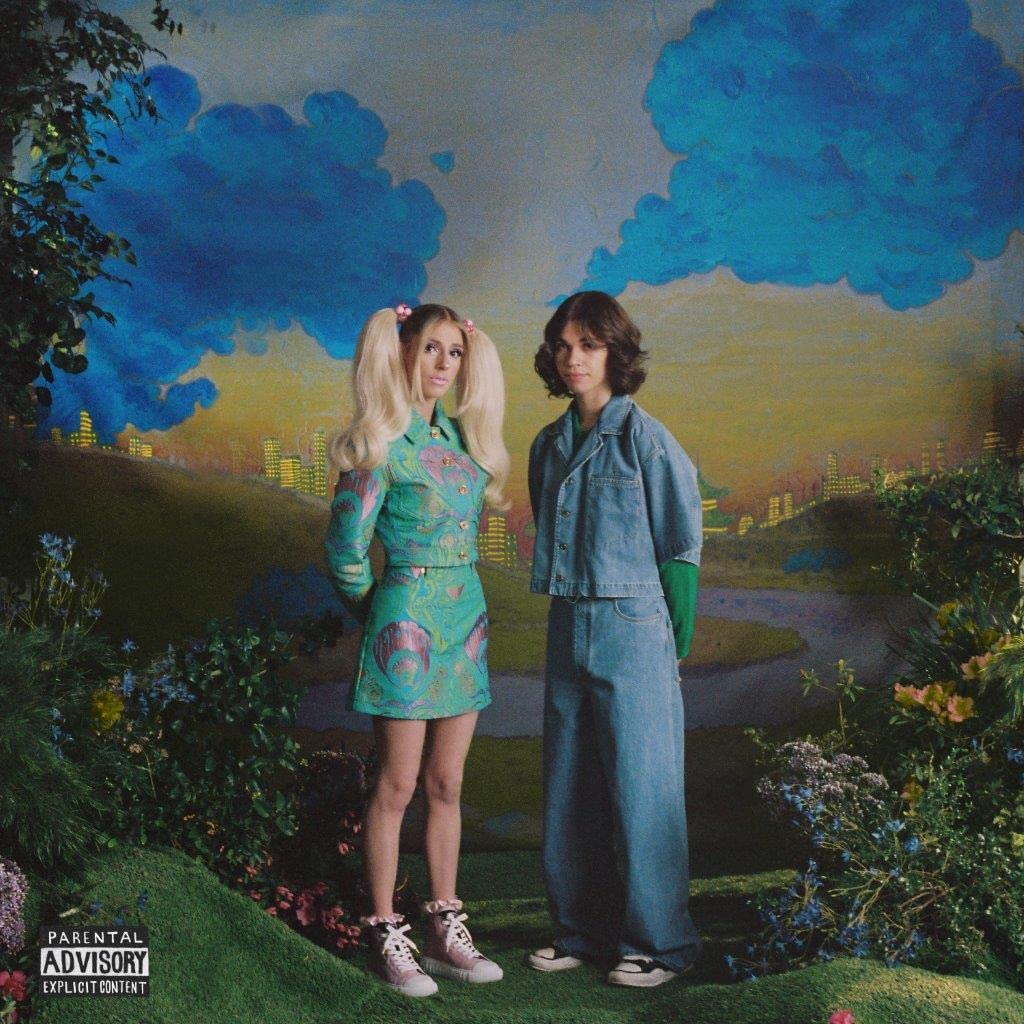
\includegraphics[width=\textwidth]{imagens-reais/not-tight/nottight.jpg}
    \caption{Original}
  \end{subfigure}%
  \hfill
  \begin{subfigure}{0.48\textwidth}
    \centering
    
\includegraphics[width=\textwidth]{imagens-reais/not-tight/compressed.png}
    \caption{Comprimida}
  \end{subfigure}%
  \hfill
  \begin{subfigure}{0.48\textwidth}
    \centering
    
\includegraphics[width=\textwidth]{imagens-reais/not-tight/decompressed-bilinear.png}
    \caption{Bilinear}
  \end{subfigure}%
  \hfill
  \begin{subfigure}{0.48\textwidth}
    \centering
    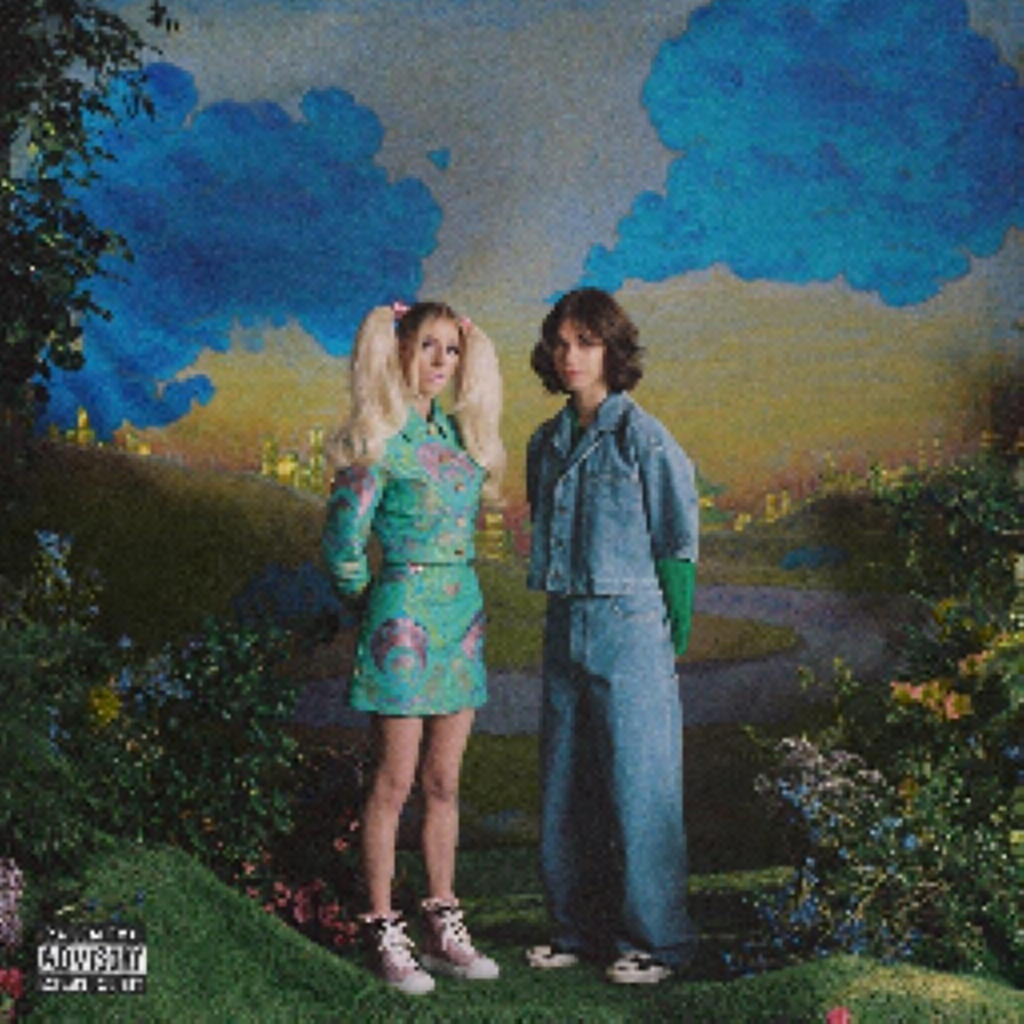
\includegraphics[width=\textwidth]{imagens-reais/not-tight/decompressed-bicubica.png}
    \caption{Bicúbica}
  \end{subfigure}
  \caption{Imagem original (1024 pixels), comprimida (256 pixels) e descomprimidas (1024 pixels)}
\end{figure}

e os erros foram 0.069800 para bilinear e 0.072539 para bicúbica.

Como há muitos detalhes na imagem original, é possível ver o
granulado na compressão e descompressões. Entretanto, o erro foi
relativamente baixo, relativo a 2 casas decimais.

\subsection{Led Zeppelin I by Led Zeppelin}

Clássico do rock dos anos 70. Mudaram por conta própria o rumo da
cena e popularizaram o estilo.

A capa é predominantemente monocromática e originalmente granulada.

Usando $k=3$ e $h=1$, as imagens resultantes foram
\clearpage
\begin{figure}[ht]
  \centering
  \begin{subfigure}{0.48\textwidth}
    \centering
    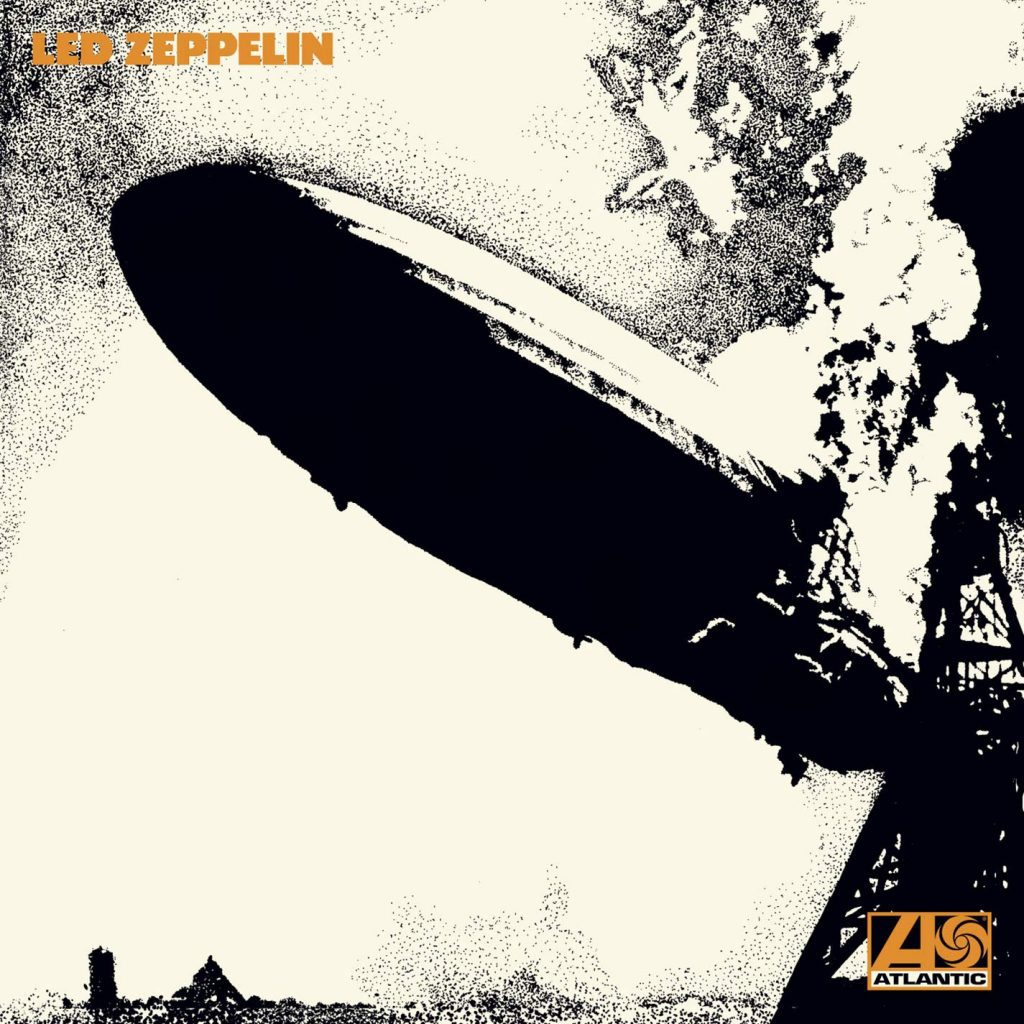
\includegraphics[width=\textwidth]{imagens-reais/led-zeppelin-1/ledzeppelini.jpg}
    \caption{Original}
  \end{subfigure}%
  \hfill
  \begin{subfigure}{0.48\textwidth}
    \centering
    
\includegraphics[width=\textwidth]{imagens-reais/led-zeppelin-1/compressed.png}
    \caption{Comprimida}
  \end{subfigure}%
  \hfill
  \begin{subfigure}{0.48\textwidth}
    \centering
    
\includegraphics[width=\textwidth]{imagens-reais/led-zeppelin-1/decompressed-bilinear.png}
    \caption{Bilinear}
  \end{subfigure}%
  \hfill
  \begin{subfigure}{0.48\textwidth}
    \centering
    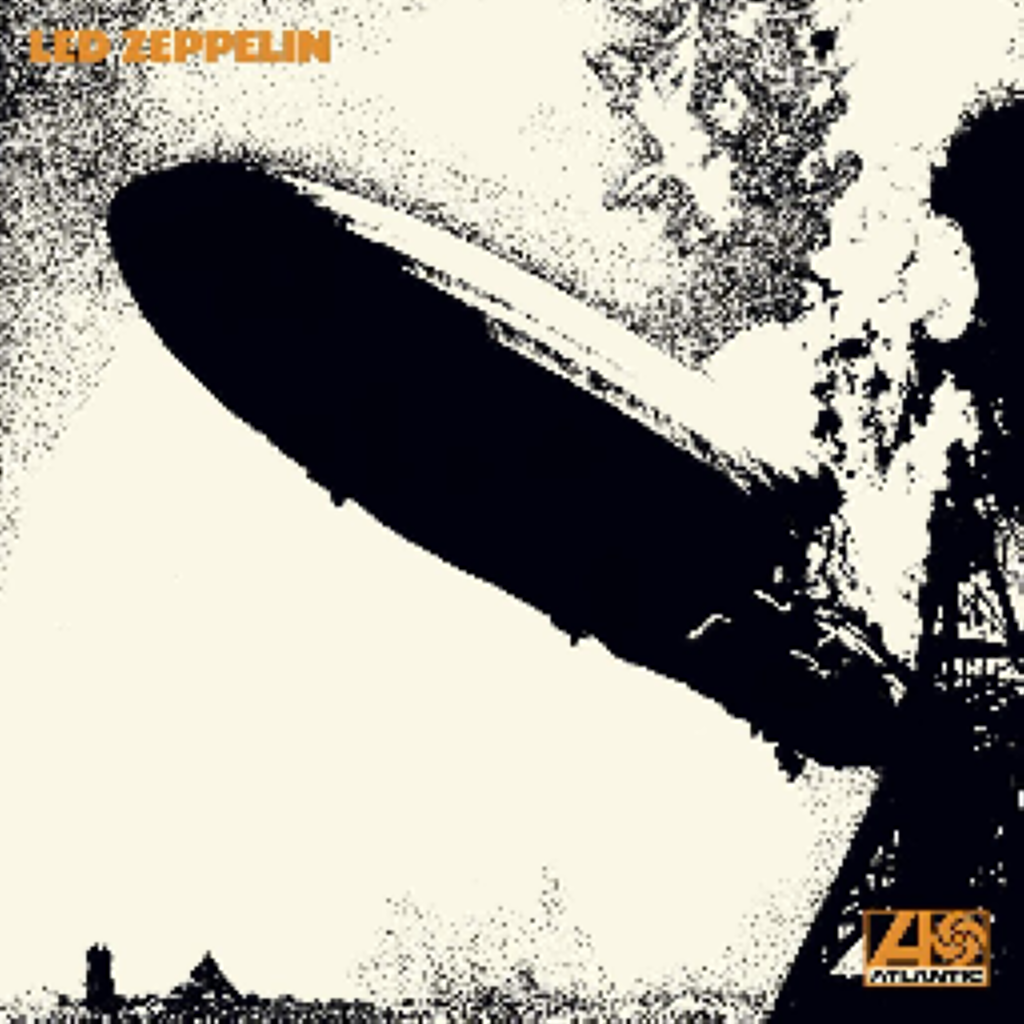
\includegraphics[width=\textwidth]{imagens-reais/led-zeppelin-1/decompressed-bicubica.png}
    \caption{Bicúbica}
  \end{subfigure}
  \caption{Imagem original (1024 pixels), comprimida (256 pixels) e descomprimidas (1024 pixels)}
\end{figure}

e os erros foram 0.1726 para bilinear e 0.1796 para bicúbica.

Ao contrário da capa de \ref{subsec:nottight}, esta é originalmente
granulada, então o efeito de granulação da compressão e descompressão é
menos perceptível. Além disso, o erro foi alto em comparação ao último,
este relativo a 1 casa decimal.

\subsection{Deep in View by Cola}

Álbum de rock indie recente, debutado em 2022. Remete ao estilo marcante
de \textit{The Strokes}, mas ainda sim com uma assinatura própria.

A capa é colorida e há linhas duras - alto contraste entre as cores e
os elementos.

Usando $k=3$ e $h=1$, as imagens resultantes foram
\clearpage
\begin{figure}[ht]
  \centering
  \begin{subfigure}{0.48\textwidth}
    \centering
    
\includegraphics[width=\textwidth]{imagens-reais/deep-in-view/deepinview.png}
    \caption{Original}
  \end{subfigure}%
  \hfill
  \begin{subfigure}{0.48\textwidth}
    \centering
    
\includegraphics[width=\textwidth]{imagens-reais/deep-in-view/compressed.png}
    \caption{Comprimida}
  \end{subfigure}%
  \hfill
  \begin{subfigure}{0.48\textwidth}
    \centering
    
\includegraphics[width=\textwidth]{imagens-reais/deep-in-view/decompressed-bilinear.png}
    \caption{Bilinear}
  \end{subfigure}%
  \hfill
  \begin{subfigure}{0.48\textwidth}
    \centering
    
\includegraphics[width=\textwidth]{imagens-reais/deep-in-view/decompressed-bicubica.png}
    \caption{Bicúbica}
  \end{subfigure}
  \caption{Imagem original (1024 pixels), comprimida (256 pixels) e descomprimidas (1024 pixels)}
\end{figure}

e os erros foram 0.1583 para bilinear e 0.1623 para bicúbica.

É perceptível a piora de definição e quadriculação de todas as bordas.
Os erros também estão relativos a 1 casa decimal.

\section{Conclusão geral}

Manipulação de imagens é uma tarefa custosa em quesito de processamento
computacional. Contudo, os métodos e a teoria numérica revelam maneiras
inteligentes para otimizar algoritmos. Uma curiosidade que estou levando
na disciplina é a codificação de algoritmos para GPUs. Quais serão as 
diferenças? Essas questões não serão respondidas agora, infelizmente.

\end{document}